% Format teze zasnovan je na paketu memoir
% http://tug.ctan.org/macros/latex/contrib/memoir/memman.pdf ili
% http://texdoc.net/texmf-dist/doc/latex/memoir/memman.pdf
% 
% Prilikom zadavanja klase memoir, navedenim opcijama se podešava 
% veličina slova (12pt) i jednostrano štampanje (oneside).
% Ove parametre možete menjati samo ako pravite nezvanične verzije
% mastera za privatnu upotrebu (na primer, u b5 varijanti ima smisla 
% smanjiti 

\documentclass[12pt,oneside]{memoir}

% Paket koji definiše sve specifičnosti mastera Matematičkog fakulteta
\usepackage{matfmaster}
%
% Podrazumevano pismo je ćirilica.
%   Ako koristite pdflatex, a ne xetex, sav latinički tekst na srpskom jeziku
%   treba biti okružen sa \lat{...} ili \begin{latinica}...\end{latinica}.
%
% Opicija [latinica]:
%   ako želite da pišete latiniciom, dodajte opciju "latinica" tj.
%   prethodni paket uključite pomoću: \usepackage[latinica]{matfmaster}.
%   Ako koristite pdflatex, a ne xetex, sav ćirilički tekst treba biti
%   okružen sa \cir{...} ili \begin{cirilica}...\end{cirilica}.
%
% Opcija [biblatex]:
%   ako želite da koristite reference na više jezika i umesto paketa
%   bibtex da koristite BibLaTeX/Biber, dodajte opciju "biblatex" tj.
%   prethodni paket uključite pomoću: \usepackage[biblatex]{matfmaster}
%
% Opcija [b5paper]:
%   ako želite da napravite verziju teze u manjem (b5) formatu, navedite
%   opciju "b5paper", tj. prethodni paket uključite pomoću: 
%   \usepackage[b5paper]{matfmaster}. Tada ima smisla razmisliti o promeni
%   veličine slova (izmenom opcije 12pt na 11pt u \documentclass{memoir}).
%
% Naravno, opcije je moguće kombinovati.
% Npr. \usepackage[b5paper,biblatex]{matfmaster}

% Pomoćni paket koji generiše nasumičan tekst u kojem se javljaju sva slova
% azbuke (nema potrebe koristiti ovo u pravim disertacijama)
\usepackage{pangrami}

% Paket koji obezbeđuje ispravni prikaz ćiriličkih italik slova kada
% se koristi pdflatex. Zakomentarisati ako na sistemu koji koristite ovaj
% paket nije dostupan ili ako ne radi ispravno.
\usepackage{cmsrb}

% Ostali paketi koji se koriste u dokumentu
\usepackage{listings} % listing programskog koda

% Datoteka sa literaturom u BibTex tj. BibLaTeX/Biber formatu
\bib{implementacija_tekst_editora_za_pisanje_koda}

% Ime kandidata na srpskom jeziku (u odabranom pismu)
\autor{Бојан Барџић}
% Naslov teze na srpskom jeziku (u odabranom pismu)
\naslov{Имплементација текст едитора за писање кода}
% Godina u kojoj je teza predana komisiji
\godina{2024}
% Ime i afilijacija mentora (u odabranom pismu)
\mentor{др Весна \textsc{Маринковић}, доцент\\ Универзитет у Београду, Математички факултет}
% Ime i afilijacija prvog člana komisije (u odabranom pismu)
\komisijaA{др Милан \textsc{Банковић}, доцент \\ Универзитет у Београду, Математички факултет}
% Ime i afilijacija drugog člana komisije (u odabranom pismu)
\komisijaB{др Иван \textsc{Чукић}, доцент\\ Универзитет у Београду, Математички факултет}
% Ime i afilijacija trećeg člana komisije (opciono)
% \komisijaC{}
% Ime i afilijacija četvrtog člana komisije (opciono)
% \komisijaD{}
% Datum odbrane (obrisati ili iskomentarisati narednu liniju ako datum odbrane nije poznat)
\datumodbrane{15. јануар 2016.}

% Apstrakt na srpskom jeziku (u odabranom pismu)
\apstr{%
\pangrami
}

% Ključne reči na srpskom jeziku (u odabranom pismu)
\kljucnereci{анализа, геометрија, алгебра, логика, рачунарство, астрономија}

\begin{document}
% ==============================================================================
% Uvodni deo teze
\frontmatter
% ==============================================================================
% Naslovna strana
\naslovna
% Strana sa podacima o mentoru i članovima komisije
\komisija
% Strana sa posvetom (u odabranom pismu)
\posveta{Мами, тати и деди}
% Strana sa podacima o disertaciji na srpskom jeziku
\apstrakt
% Sadržaj teze
\tableofcontents*

% ==============================================================================
% Glavni deo teze
\mainmatter
% ==============================================================================

% ------------------------------------------------------------------------------
\chapter{Увод}
% ------------------------------------------------------------------------------
\pangrami

\section{Текст едитори}

\paragraph{}
Текст едитор је програм за измену текстуалних датотека. Најчешћи типови датотека
који се измењују коришћењем ових програма су једноставне текстуалне датотеке, 
датотеке које садржe изворни код, код језика за означавање као и конфигурационе датотеке. 
Неки од најпознатијих оваквих програма су \begin{latinica}Visual Studio Code\end{latinica} \cite{VSC}, 
\begin{latinica}Notepad\end{latinica} \cite{Notepad}, \begin{latinica}Notepad++\end{latinica} 
\cite{Notepad++}, \begin{latinica}VIM\end{latinica} \cite{VIM} и \begin{latinica}Emacs\end{latinica} \cite{Emacs}.

\paragraph{}
Постоји више врста текст едитора. Имамо едиторе једноставног текста, где информација
о датотеци предсавља само текст. Док такође постоје и едитори богатог текста, где
информација о датотеци поред текста садржи и неке додатне информације везано за изглед
текста (фонт, величина фонта, боја текста, маргине). Ми ћемо се у овом раду бавити искључиво
едиторима једноставног текста.

\section{Структуре података у текст едиторима}
\paragraph{}
Пошто текст у датотеци можемо посматрати као линеарни низ карактера, 
тако и сваку измену над тим текстом можемо посматрати као додавање текста у
неки део низа или брисање подниза текста. Када бисмо сав текст једне датотеке
које смо отворили чували као један низ карактера, видели бисмо да су горе наведене 
операције јако временски скупе (линеарне сложености) и да њихово стално извршавање
над неким великим текстом би имало за последицу изузетну неефикасност текст едитора.
Да би се овај проблем превазишао измишљене су разне структуре података које ове операције
врше ефикасније. Најпознатије овакве структуре су бафер са размацима 
(енг. \begin{latinica}gap buffer\end{latinica}), уже (енг. \begin{latinica}rope\end{latinica}) 
и табела делова (енг. \begin{latinica}piece table\end{latinica}).

\subsection{Бафер са размацима}
\paragraph{}
Бафер са размацима (енг. \begin{latinica}gap buffer\end{latinica}) је једноставна структура
података која се заснива на једноставној идеји да постоји један линеаран низ чија је средина
"празна", док се са леве и десне стране налази текст. Како ми вршимо измене над неким делом 
текста тако се средина "помера" превлачењем последњег елемента леве стране на почетак десне
или обрнуто. Када се бафер попуни (размак није довољно велики за нову операцију), тада се 
алоцира нови бафер већих димензија, најчешће дупло већи, и у њега се копира текст из старог
бафера.
\paragraph{}
Што се тиче ефикасности ове структуре, у односу на класичан низ, бафер са размацима је доста 
ефикаснији јер немамо нову реалокацију низа при свакој измени. Ефикасност уметања и 
брисања зависи највише од тога колики је размак између индекса на коме желимо да 
извршимо измену текста и леве или десне границе размака. Ако је размак већ на потребној позицији, 
временска сложеност је константна. Међутим, ако је размак на једном крају а ми желимо да 
мењамо други крај текста сложеност ће бити линеарна. У просечном случају временска 
сложеност је константна, јер најчешће пишемо карактере један за другим. 
Једина операција која је преостала је алоцирање новог низа, која је линеарне сложености.

\paragraph{}
Ова структура је једноставна за имплементацију и често се користи за једноставне текстуалне
уносе. Познати текст едитор \begin{latinica}Emacs\end{latinica} \cite{Emacs} користи 
ову структуру у својој имплементацији. На слици \ref{fig:gap_buffer} приказана је илустрација
рада бафера.

\begin{figure}[!ht]
  \centering
  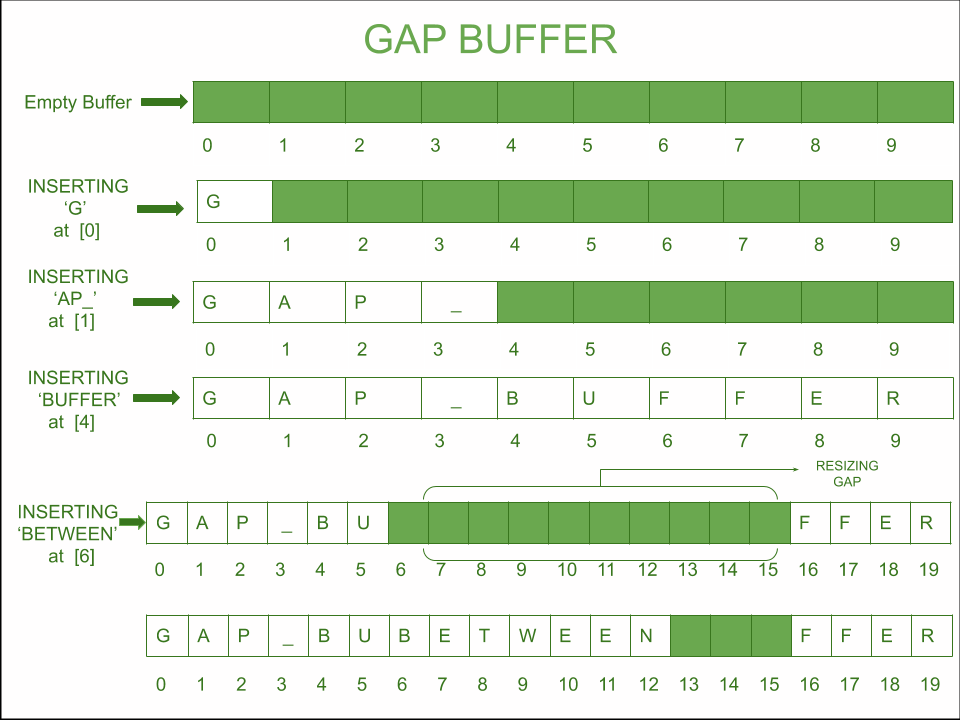
\includegraphics[width=1.0\textwidth]{images/gap_buffer.png}
  \caption{Илустрација бафера са размаком}
  \label{fig:gap_buffer}
\end{figure}


% ------------------------------------------------------------------------------
\chapter{Разрада}
\label{chp:razrada}
% ------------------------------------------------------------------------------

\pangrami

\pangrami

% ------------------------------------------------------------------------------
\chapter{Закључак}
% ------------------------------------------------------------------------------
\pangrami

\pangrami

% ------------------------------------------------------------------------------
% Literatura
% ------------------------------------------------------------------------------
\literatura

% ==============================================================================
% Završni deo teze i prilozi
\backmatter
% ==============================================================================

% ------------------------------------------------------------------------------
% Biografija kandidata
\begin{biografija}
\textbf{Вук Стефановић Караџић} (\emph{Тршић, 26. октобар/6. новембар
  1787. — Беч, 7. фебруар 1864.}) био је српски филолог, реформатор
српског језика, сакупљач народних умотворина и писац првог речника
српског језика.  Вук је најзначајнија личност српске књижевности прве
половине XIX века. Стекао је и неколико почасних доктората.
Учествовао је у Првом српском устанку као писар и чиновник у
Неготинској крајини, а након слома устанка преселио се у Беч,
1813. године. Ту је упознао Јернеја Копитара, цензора словенских
књига, на чији је подстицај кренуо у прикупљање српских народних
песама, реформу ћирилице и борбу за увођење народног језика у српску
књижевност. Вуковим реформама у српски језик је уведен фонетски
правопис, а српски језик је потиснуо славеносрпски језик који је у то
време био језик образованих људи. Тако се као најважније године Вукове
реформе истичу 1818., 1836., 1839., 1847. и 1852.
\end{biografija}
% ------------------------------------------------------------------------------

\end{document} 